\chapter{Theoretical concepts}\label{cha:theory}


\section{Measurment of the charge radius of the proton}\label{sec:proton_radius}
The proton is a baryon, a composite particle made of up two up quarks and one down quark.
From this follows that the proton is not a point particle,but has an internal sturucture.
The internal  distrubiton of the charge defines the charge radius of the proton.
\subsection{Previous measurements of the proton radius}
The charge radius of the proton has been massured several times before with different methods.
The two premier methods are electron proton scattering experiments and the Lamb shift in muonic and ordinary hydrogen.
The results of these measurements differ by five standard deviations as shown in figure \ref{fig:previous_proton_radius},
this has given rise to the so called proton radius puzzle \autocite{ProposalAmber}.
\begin{figure}[H]
	\centering
	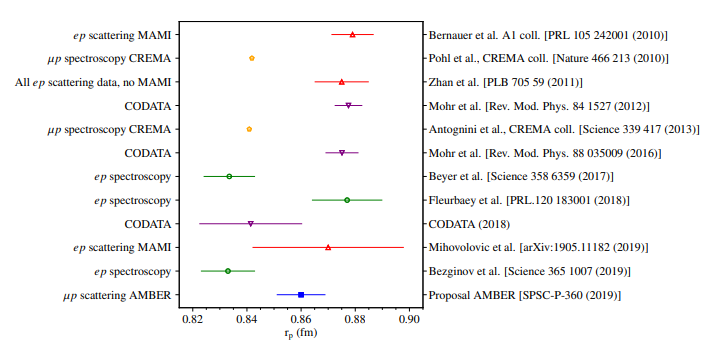
\includegraphics[width=0.8\textwidth]{PreviousmeausrementsProtonradius.png}
	\caption{Previous measurements of the proton radius from electron scattering experiments and the Lamb shift in muonic and ordinary hydrogen \autocite{ProposalAmber} }
	\label{fig:previous_proton_radius}
\end{figure}






\subsection{Measurment of the proton radis with elastic scattering of muons on protons}
The Amber experiment at CERN aims to reslove the proton radius puzzle, by measuring the elastic scattering of muons on protons.

The first order cross section for the elastic scattering of muons on a proton target is \autocite{intentAmber}
INSERT: maybe  here more explantation 
\begin{equation}
\label{eq:cross_section}
\frac{d\sigma}{dQ^2} = \frac{\pi \alpha^2}{Q^4 m_p^2 p_\mu^2} \bigg[ \left( G_E^2 + \tau G_M^2 \right) \frac{ 4E_\mu^2 m_p^2 - Q^2 (s - m_\mu^2)}{1 + \tau }  - G_M^2 \frac{ 2m_\mu^2 Q^2 - Q^4}{2} \bigg]
\end{equation}
with  $Q^2 = -q^2$, $\tau = Q^2 / 4m_p^2$, $s = (p_\mu + p_p)^2$, $p_\mu$ the momentum of the muon, $p_p$ the momentum of the proton, $m_p$ the mass of the proton,
 $m_\mu$ the mass of the muon, $E_\mu$ the energy of the muon, $G_E$ the electric form factor of the proton,
  $G_M$ the magnetic form factor of the proton and $\alpha$ the fine structure constant.
  INSERT: maybe  here more explantation 
Through determening the form factors $G_E$ and $G_M$, the charge radius of the Proton can be claculated with the following equation \autocite{intentAmber}
\begin{equation}
\label{eq:charge_radius}
r_p^2 = -6 \frac{dG_E}{dQ^2} \bigg|_{Q^2 = 0}
\end{equation}

\section{General setup  at AMBER}\label{sec:general_setup}
To determine the magentic and electric form factors of the proton and thus the charge radius of the Proton, the experimental cross section of the elastic scattering of muons on protons has to be measured.
The general setup of the Amber experiment is shown in figure \ref{fig:amber_setup}.
\begin{figure}[h]
	\centering
	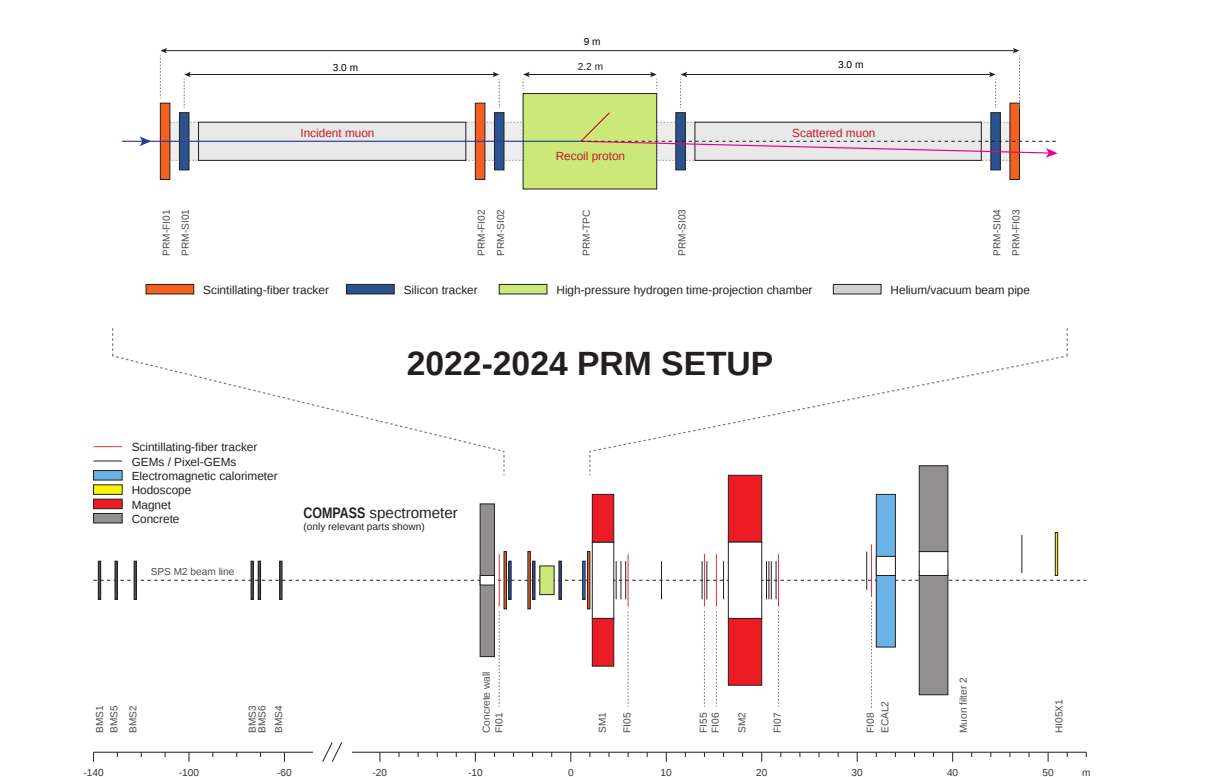
\includegraphics[width=1.2\textwidth]{OverviewSetupAmber.png}
	\caption{General setup of the Amber experiment with new detectors for PR-Measurments,INSERT:BETTER DISCRIPTION \autocite{ProposalAmber}}
	\label{fig:amber_setup}
\end{figure}
INSERT: MAYBE FLUX;ENERGY
The incoming muon beam is scattered on a pressurized hydrogen gas target, located in the Time Projection Chamber (TPC), which also acts as the detector for the recoil path of the proton.
The reconstruction of the path of the muon is achieved through the usage of two detector types.


